\documentclass{article}

\usepackage[italian]{babel}     %testi autogenerati italiano
\usepackage{graphicx}           %per importare immagini
\usepackage{geometry}           %per gestire margini e spostamenti
\usepackage[raggedright]{titlesec}
\geometry {
    top=20mm,
    bmargin=20mm,
}
\usepackage{array}              %per colonne di width fissata
\usepackage{subcaption}         %tabelle divise
\usepackage{hyperref}           %links
\hypersetup{
    colorlinks=true,
    linkcolor=black,
    urlcolor=blue
}
%\usepackage[bottom]{footmisc}   %footnotes fissate a piè pagina
\usepackage{booktabs}           %per tabitem in tabular
\newcommand{\tabitem}{~~\llap{\textbullet}~~}
\renewcommand*{\thefootnote}{[\arabic{footnote}]}

\begin{document}

\setlength\parindent{0pt} %noindent automatico
\setlength\parskip{1em}

\begin{titlepage}
	\centering
	\hrule
	
	\vspace{6,5cm}
	{\Huge \textbf{Home Challenge \#3\\
		2020/21}\\}
		
		\vspace{0,5cm}
		\large {Prof. Cesana Matteo}
		
		\vspace{2,5cm}
		{
			\large
			\begin{tabular}{c c}
				Shalby Hazem Hesham Yousef & (Personal Code: 10596243) \\
			\end{tabular}
			
		}
		\vspace{4cm}
		
		\normalsize{10 May 2021}
		\vspace{0,2cm}
		
		\centering\hspace{0,2cm}
\includegraphics[scale=0.6]{./logo.png}
		\vspace{0,5cm}
		\hrule
		
		\end{titlepage}
		
		\pagebreak
		
		\pagebreak
		
		\section{Preparation} %1
        Move the three motes to put every device in communication with the other two. 
        \begin{center}
        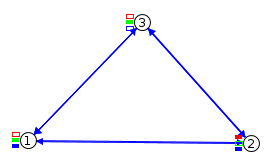
\includegraphics{./mote_screen.png}            
        \end{center}

        \section{Results} %2
        The First \texttt{20} values\footnote{Each value represents the status of the mote after the reception of a message} of the LEDs of mote \texttt{\#2} in binary form are the following\footnote{The binary form is $b_2 b_1 b_0$  where \texttt{$b_i$} is \texttt{1} if the i-th LED is ON and \texttt{0} if is OFF }:
        \begin{center}
            \texttt{000\footnote{Here a reset has been done because the received message has \texttt{(counter mod 10) == 0}}, 100, 101, 001, 101, 001, 101, 001, 000, 100, 000, 100, 000, 100, 101, 000\footnote{Here a reset has been done because the received message has \texttt{(counter mod 10) == 0}}, 100, 000, 100, 000}
        \end{center}
        Since the considered Mote receive message from the Mote \texttt{3} (\texttt{5Hz}) and Mote 1 (\texttt{1Hz}), we had a Cycle in which in any iteration we receive \texttt{5} messages from Mote \texttt{3} and \texttt{1} from Mote \texttt{1}.\\
        The result starts with two message and not five of Mote \texttt{3} because the two devices (ID.\texttt{1} and ID.\texttt{3}) have different boot time, but than the cycle described before is respected as long as the two devices run.
        
        \section{Implementation} %3
        The only thing worthy of note is the usage of three variable of type bool to get the status of three LEDs. This has been required because the Leds.get() function doesn't work as described in the documentation.
		\\\\\pagebreak
		\pagebreak
		\clearpage
\end{document}